%!TEX root = ../Thesis.tex
\chapter{System Design}\label{cha:system_design}
%

\textcolor{red}{The method chapter should describe in detail which activities you undertake to answer the research questions presented in the introduction, and why they were chosen. This includes detailed descriptions of experiments,surveys, computations, data analysis, statistical tests etc.}

We will design a system which will help us answer the following \textbf{research question}:
\begin{tcolorbox}

\begin{displayquote}
    $\mathbf{RQ}$\textbf{:} Is there a correlation between the objective measures pixel accuracy,  and Dice Coefficient and the subjective measures of satisfaction, level of artifacts and level of annoyance in the machine learning based foreground extracted processed videos?
\end{displayquote}

\end{tcolorbox}


To help us investigate the research question, we also form some supporting hypotheses. We expect that the videos which gets a low score on the objective measures, also will receive a poor score subjectively. 
\begin{tcolorbox}
\begin{displayquote}
    $\mathbf{H_1}$\textbf{:} The videos with poor objective statistics will also receive poorer rating from the subjective testing.
\end{displayquote}
\end{tcolorbox}

Another interesting subject, is to see if the videos which received a good objective testing, will be matched with a good rating from the participants

\begin{tcolorbox}
\begin{displayquote}
    $\mathbf{H_2}$\textbf{:} The videos with good objective statistics will also receive a good rating from the subjective testing.
\end{displayquote}
\end{tcolorbox}

In the coming sections we go through how we designed a system which tried to test this. 



\section{Video setup}
We will create a system consisting of several parts. The basic construction will be set of foreground videos in front of a green screen (figure \ref{fig:videos}a), where we try to create situations which we imagine could reflect some real world usage. The resulting video will be edited using chroma key compositing to remove the background (figure \ref{fig:videos}b). Further on, the video will be inserted onto different kind of background videos (figure \ref{fig:videos}c). This video will finally be processed by our machine learning based foreground extractor, which will output our segmented silhouette extraction (figure \ref{fig:videos}d). 

\begin{figure}[H]
  \centering
  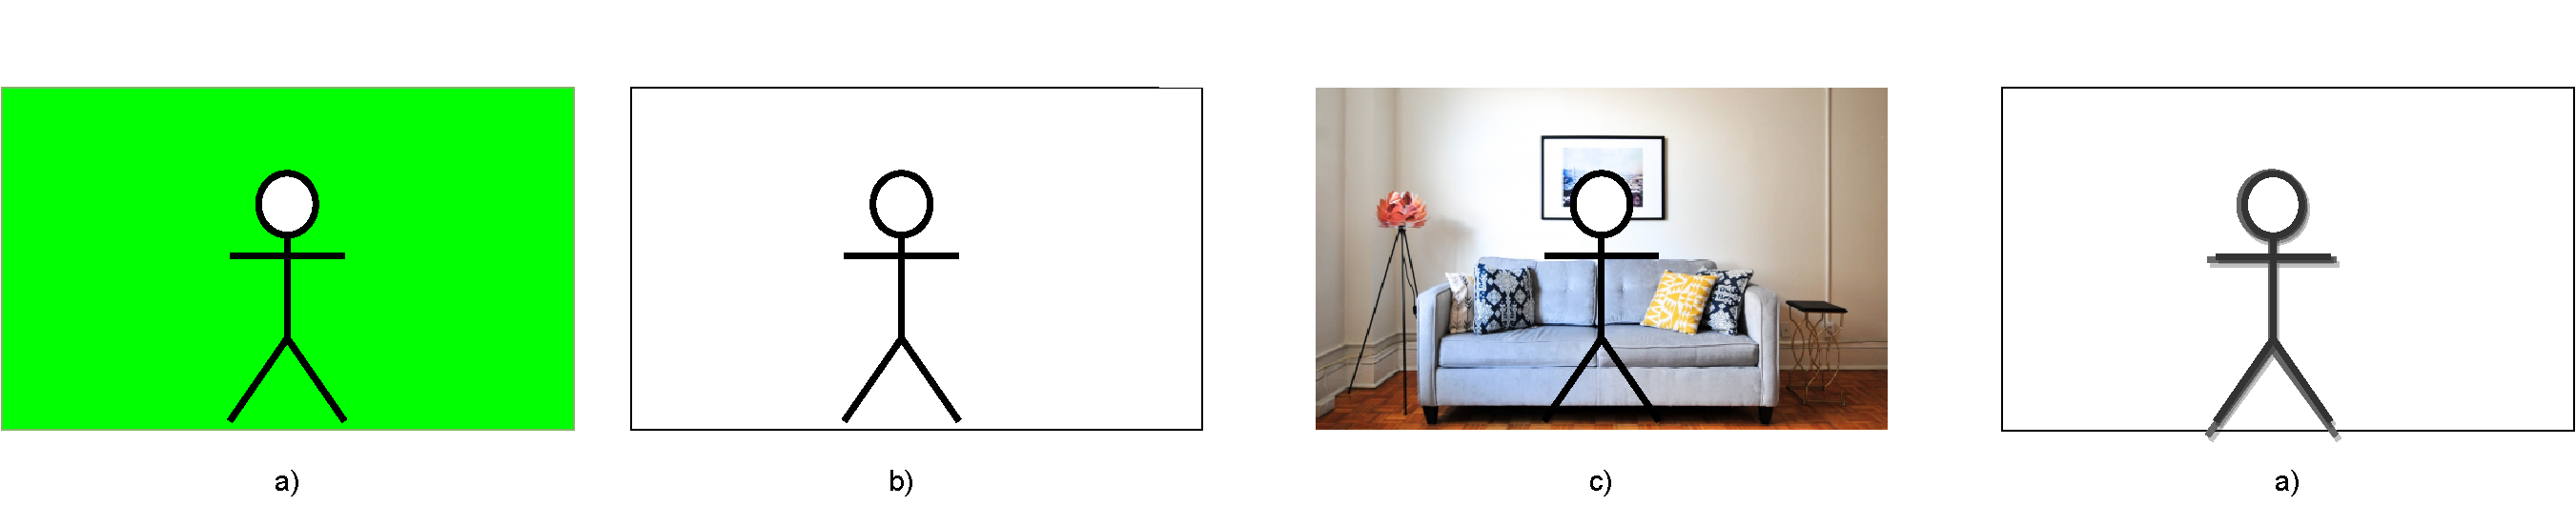
\includegraphics[width=\textwidth]{img/video_setup/video_system_design.pdf}
  \caption{Phases of video system design}
  \label{fig:videos}
\end{figure}

We will create three different backgrounds, described in \autoref{sec:backgrounds}, along with four different type of foreground videos, described in \autoref{sec:foregrounds}. By combining the background and foreground videos we will have a total of twelve (12) videos to run our objective and subjective analysis. Each video will have a duration of ten (10) seconds filmed at 30 fps. This will result in each video having 300 frames.

\subsection{Backgrounds}\label{sec:backgrounds}

An on-site shot of each background shot can be found in \autoref{cha:appendix-backgrounds}. Each of the background shots in the following section has been taken from frame 150 of the 300 frames video.

\subsubsection{Simple white wall}
A simple white wall with typical hall way lighting was selected to try to give the algorithm a ''simple'' task where the foreground would be in stark contrast to the background.

\begin{figure}[H]
    \centering
    
\includegraphics[width=0.7\textwidth]{img/video_frame_150/BG_White-Wall_150.jpg}
    \caption{Frame 150 from the simple white wall background video}
    \label{fig:background_white_wall}
\end{figure}


\subsubsection{Complex wall with different colours and textures}
A step up from the simple white wall, which will maybe be more similar to the tasks the algorithm will be put through on a regular. This background got a lot of different colors and textures from the plants, concrete wall and tiling on the floor.

\begin{figure}[H]
    \centering
    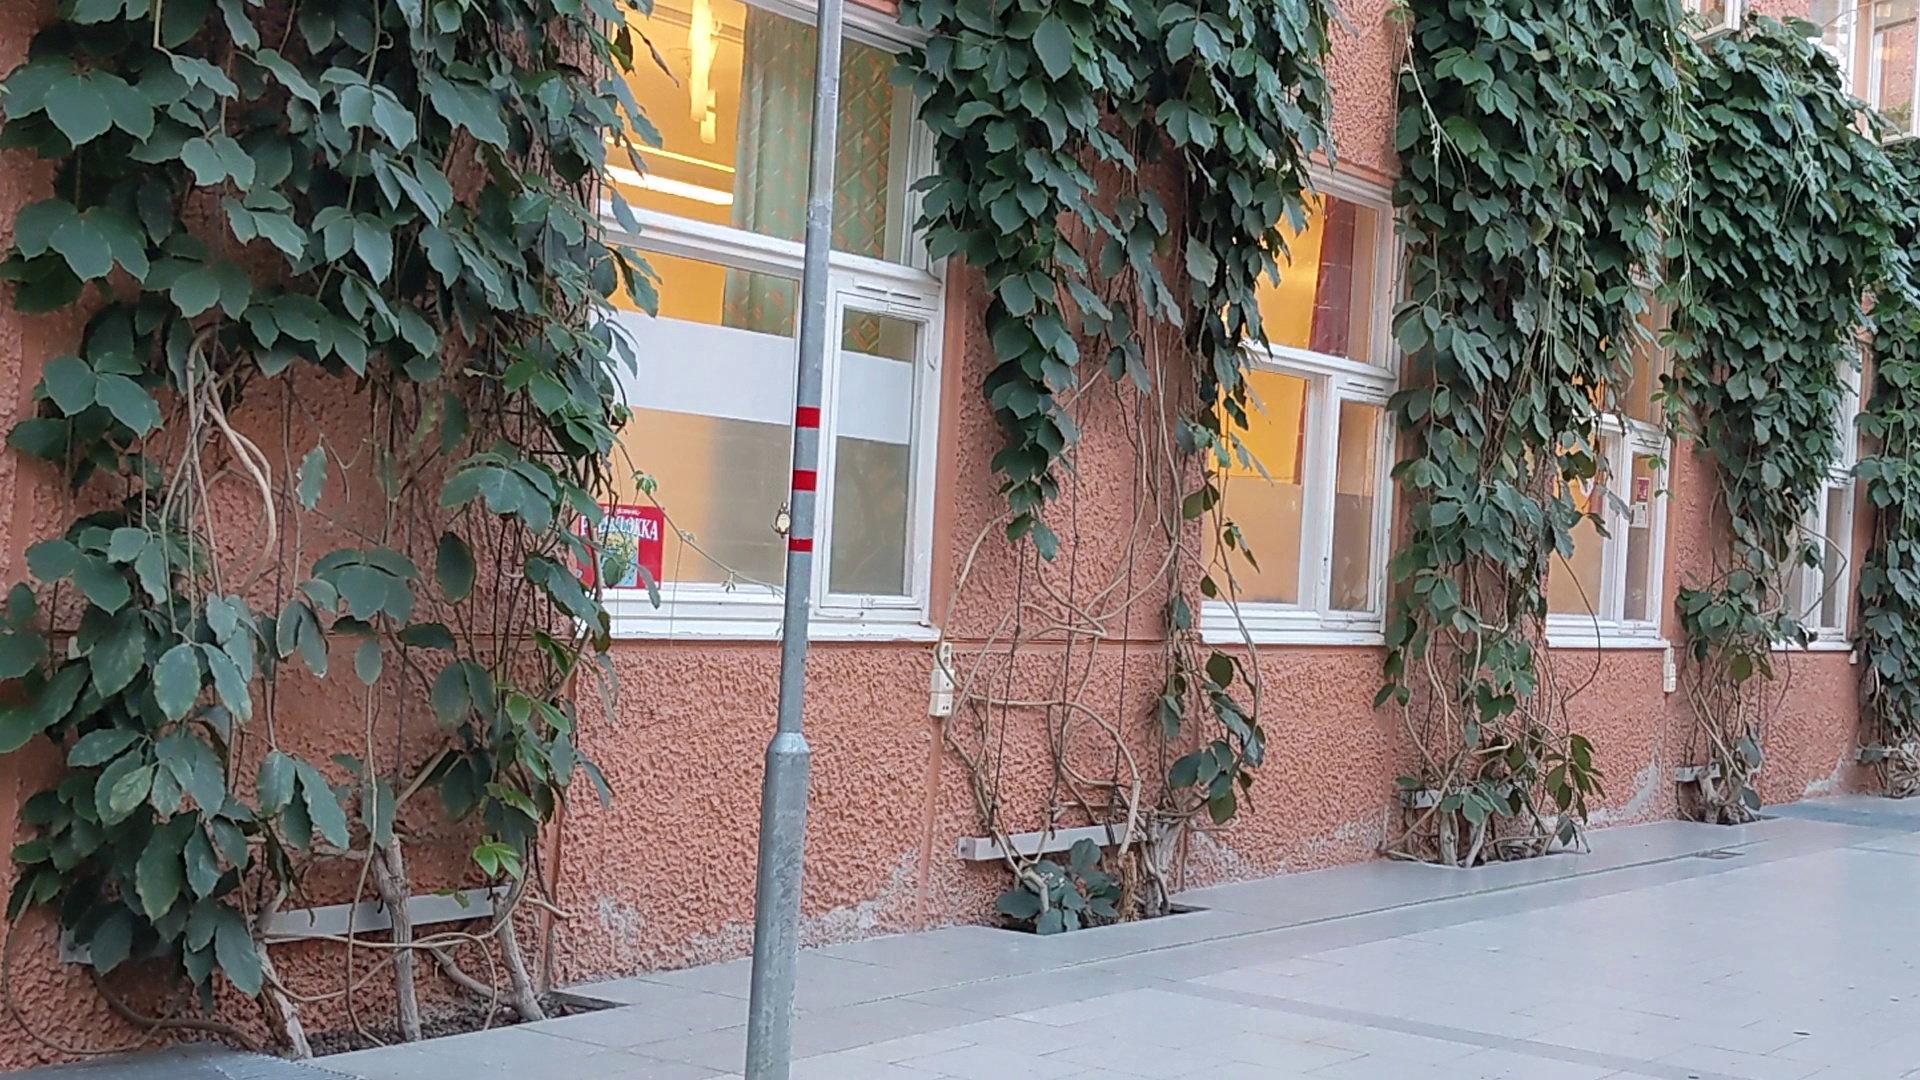
\includegraphics[width=0.7\textwidth]{img/video_frame_150/BG_Complex_150.jpg}
    \caption{Frame 150 from the complex wall background video}
    \label{fig:background_complex_wall}
\end{figure}

\subsubsection{Background with windows}
Also a similar shot to the complex wall, sharing a lot of the same characteristics, but with a bright shining window opening to the right back. This gives the algorithm a challenge with the different types of exposures in the image. This video also contains some movements from the people in the shot, which leads to this being the most dynamic shot. 

\begin{figure}[H]
    \centering
    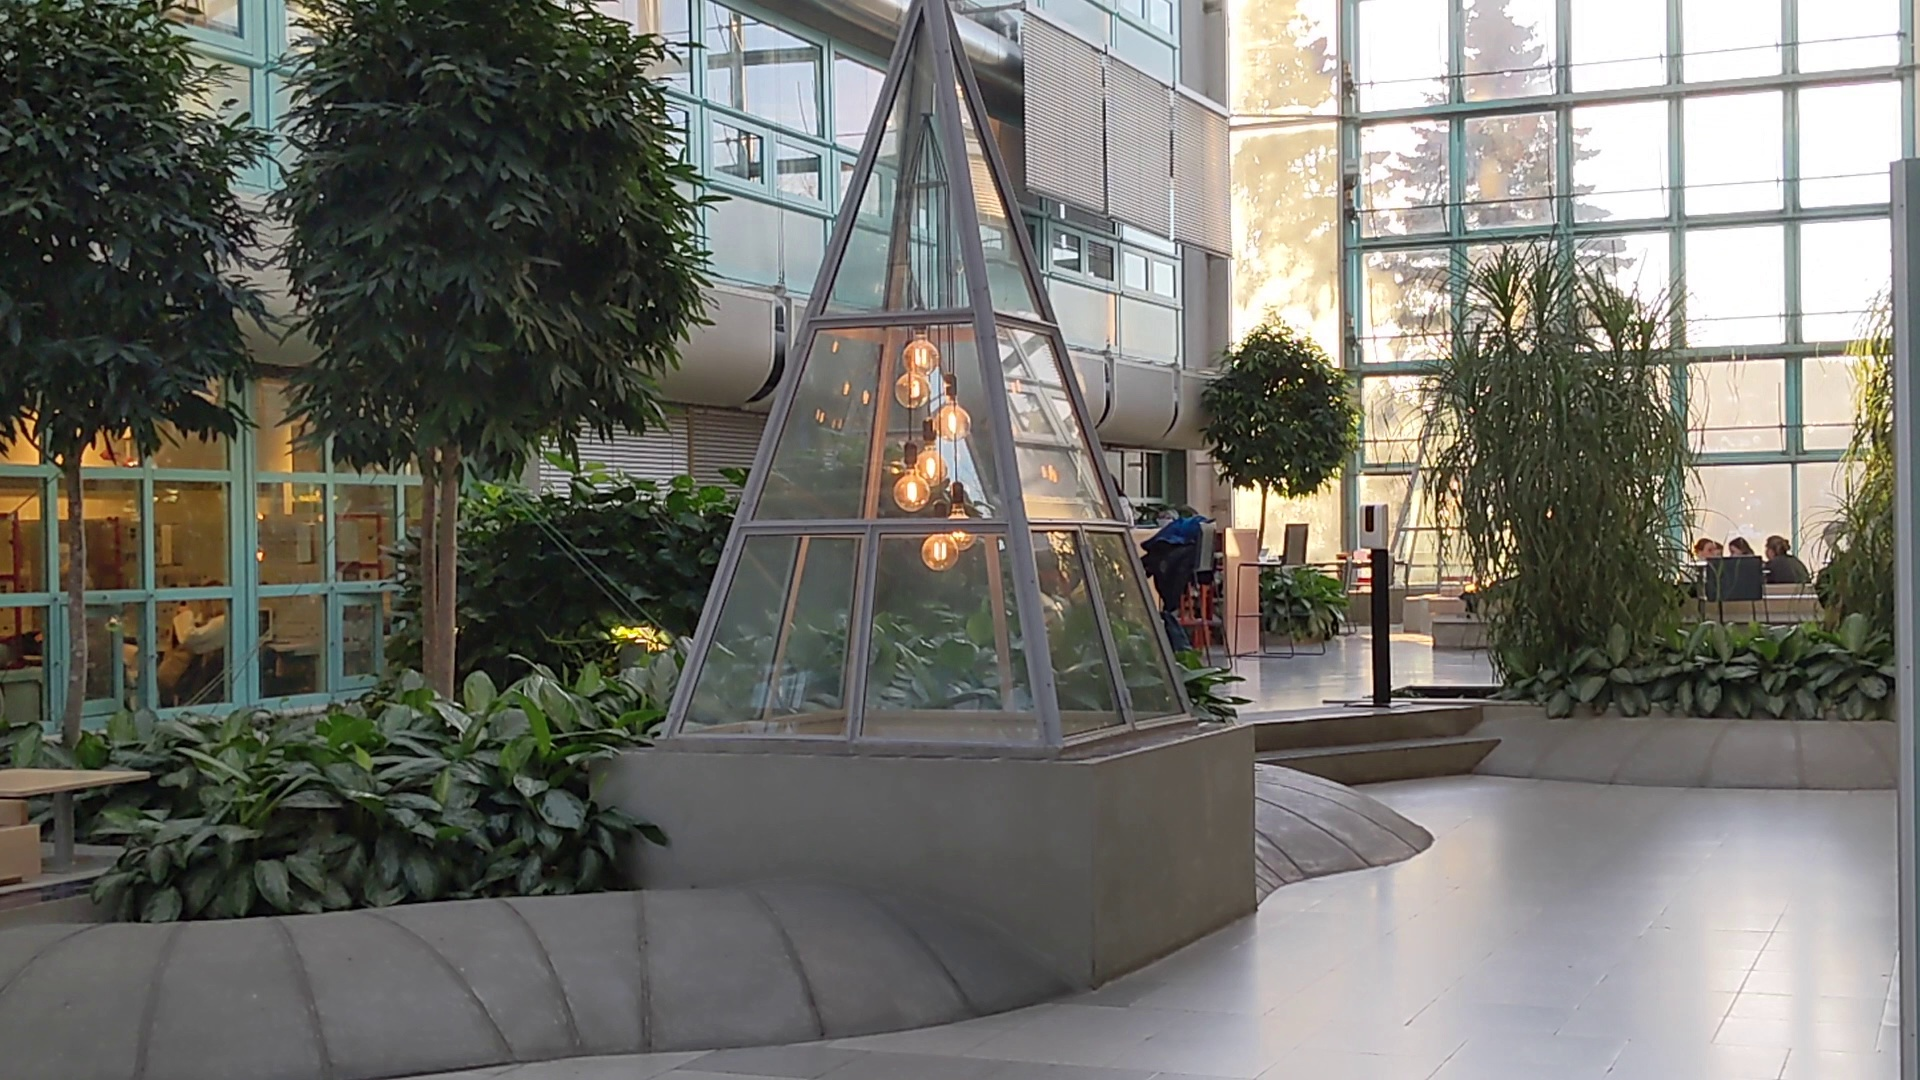
\includegraphics[width=0.7\textwidth]{img/video_frame_150/BG_Window_150.jpg}
    \caption{Frame 150 from the window wall background video}
    \label{fig:background_window_wall}
\end{figure}

\subsection{Foregrounds}\label{sec:foregrounds}
The foreground videos were constructed inside the Sense-IT laboratory at NTNU. \autoref{fig:placement} illustrates the setup and how the gear, described in \autoref{sec:hardware}, was placed. 

The placement of the ring lights were decided by trial and error to try to minimise the shadow casting from the actor onto the green screen. This step was important for easier chroma key post processing.

\begin{figure}[H]
  \centering
  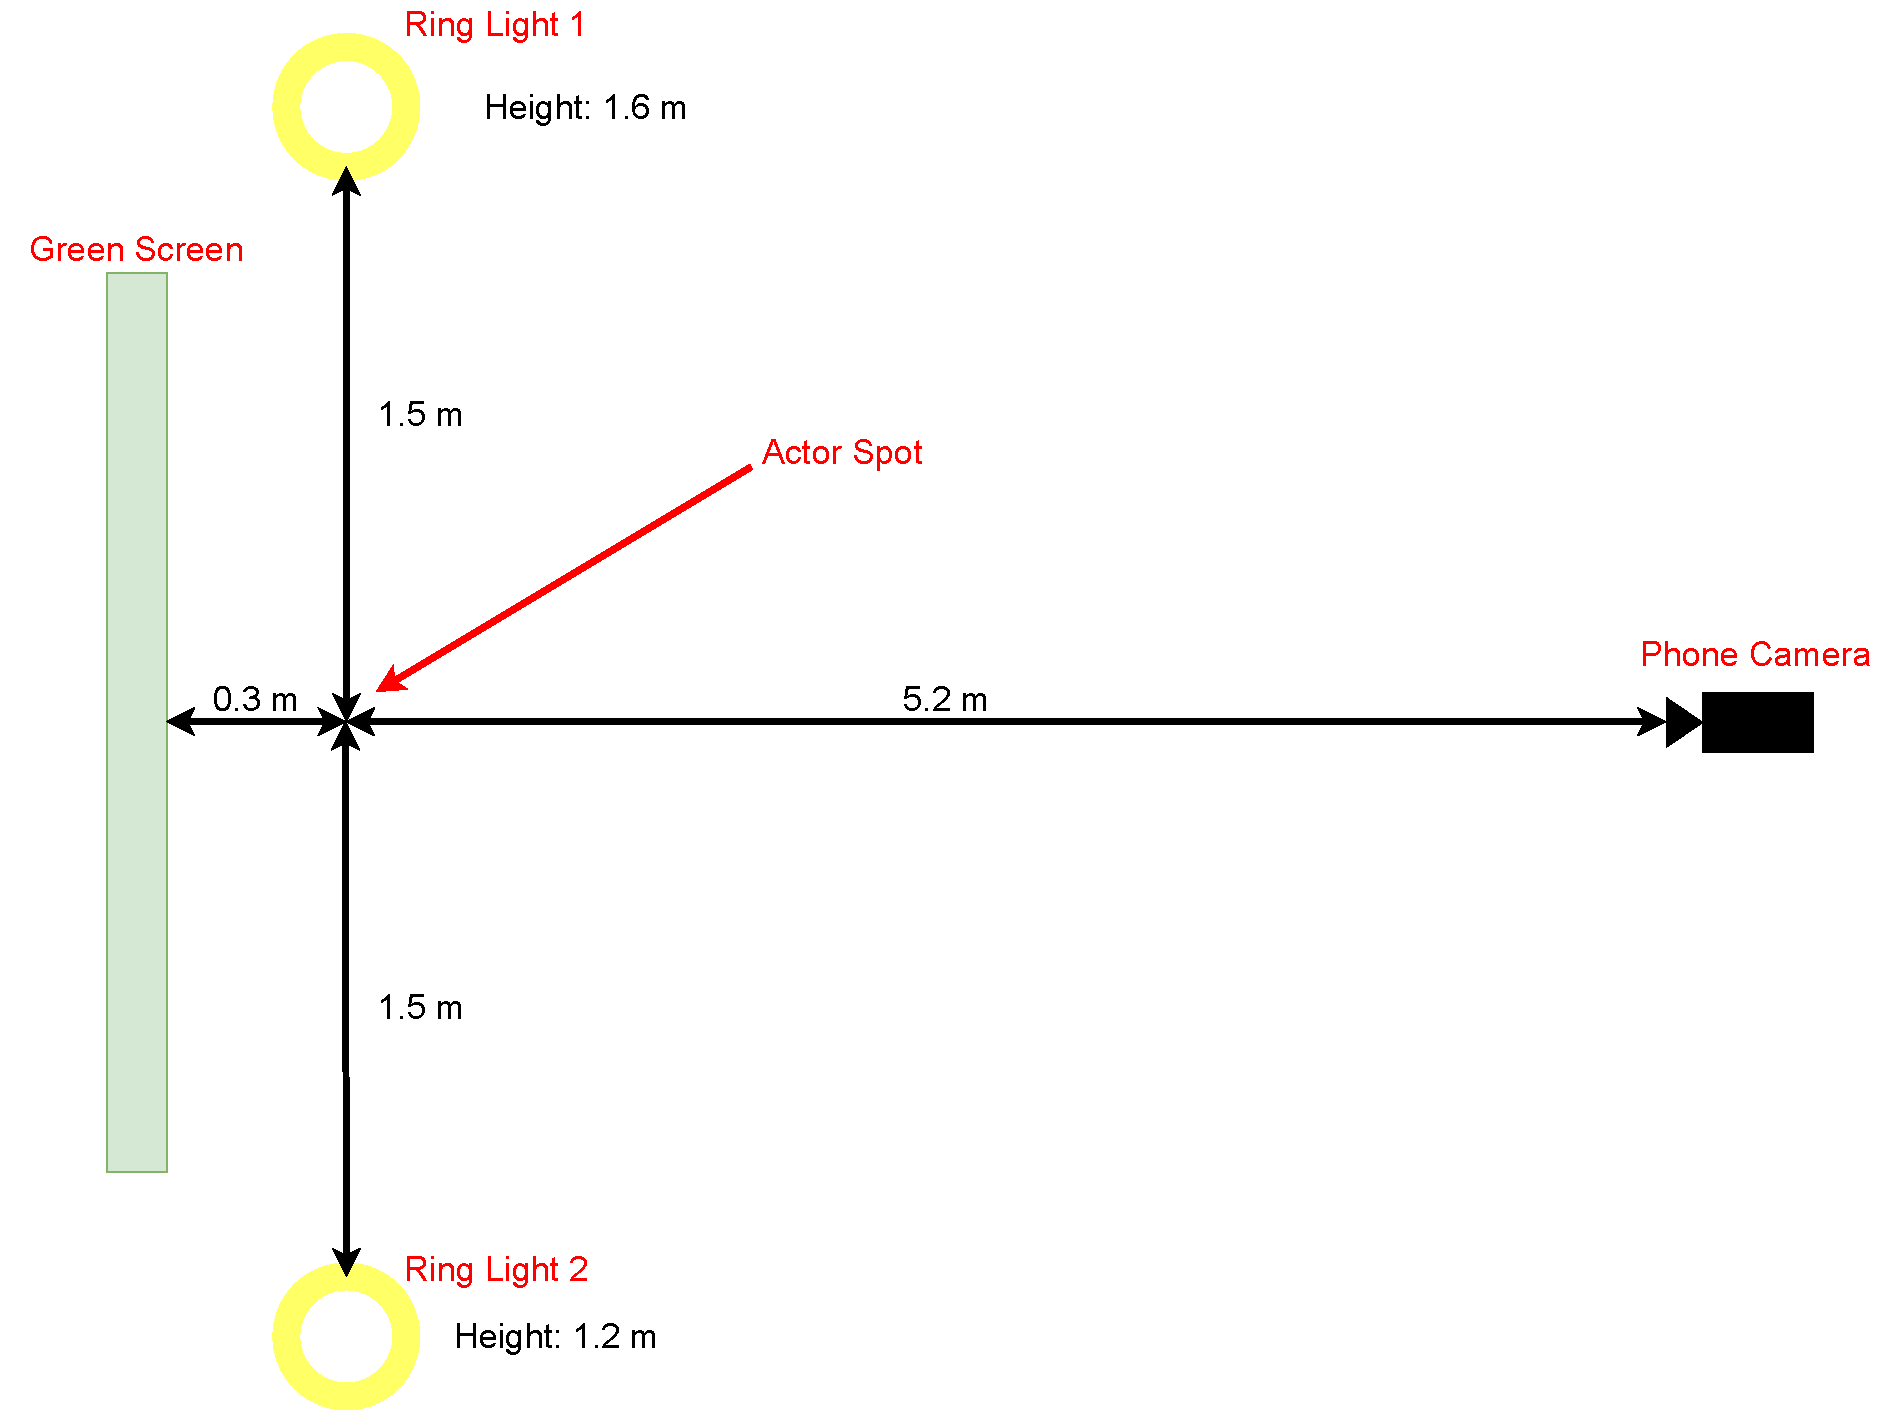
\includegraphics[width=\textwidth]{img/video_setup/placement.pdf}
  \caption{Placement of gear in the Sense-IT laboratory for the foreground shots}
  \label{fig:placement}
\end{figure}

\subsubsection{Person counting ten fingers}
This foreground was constructed to evaluate how well the machine learning algorithm handles the spacing between the fingers and how well it manages to segment these small areas.

\begin{figure}[H]
    \centering
    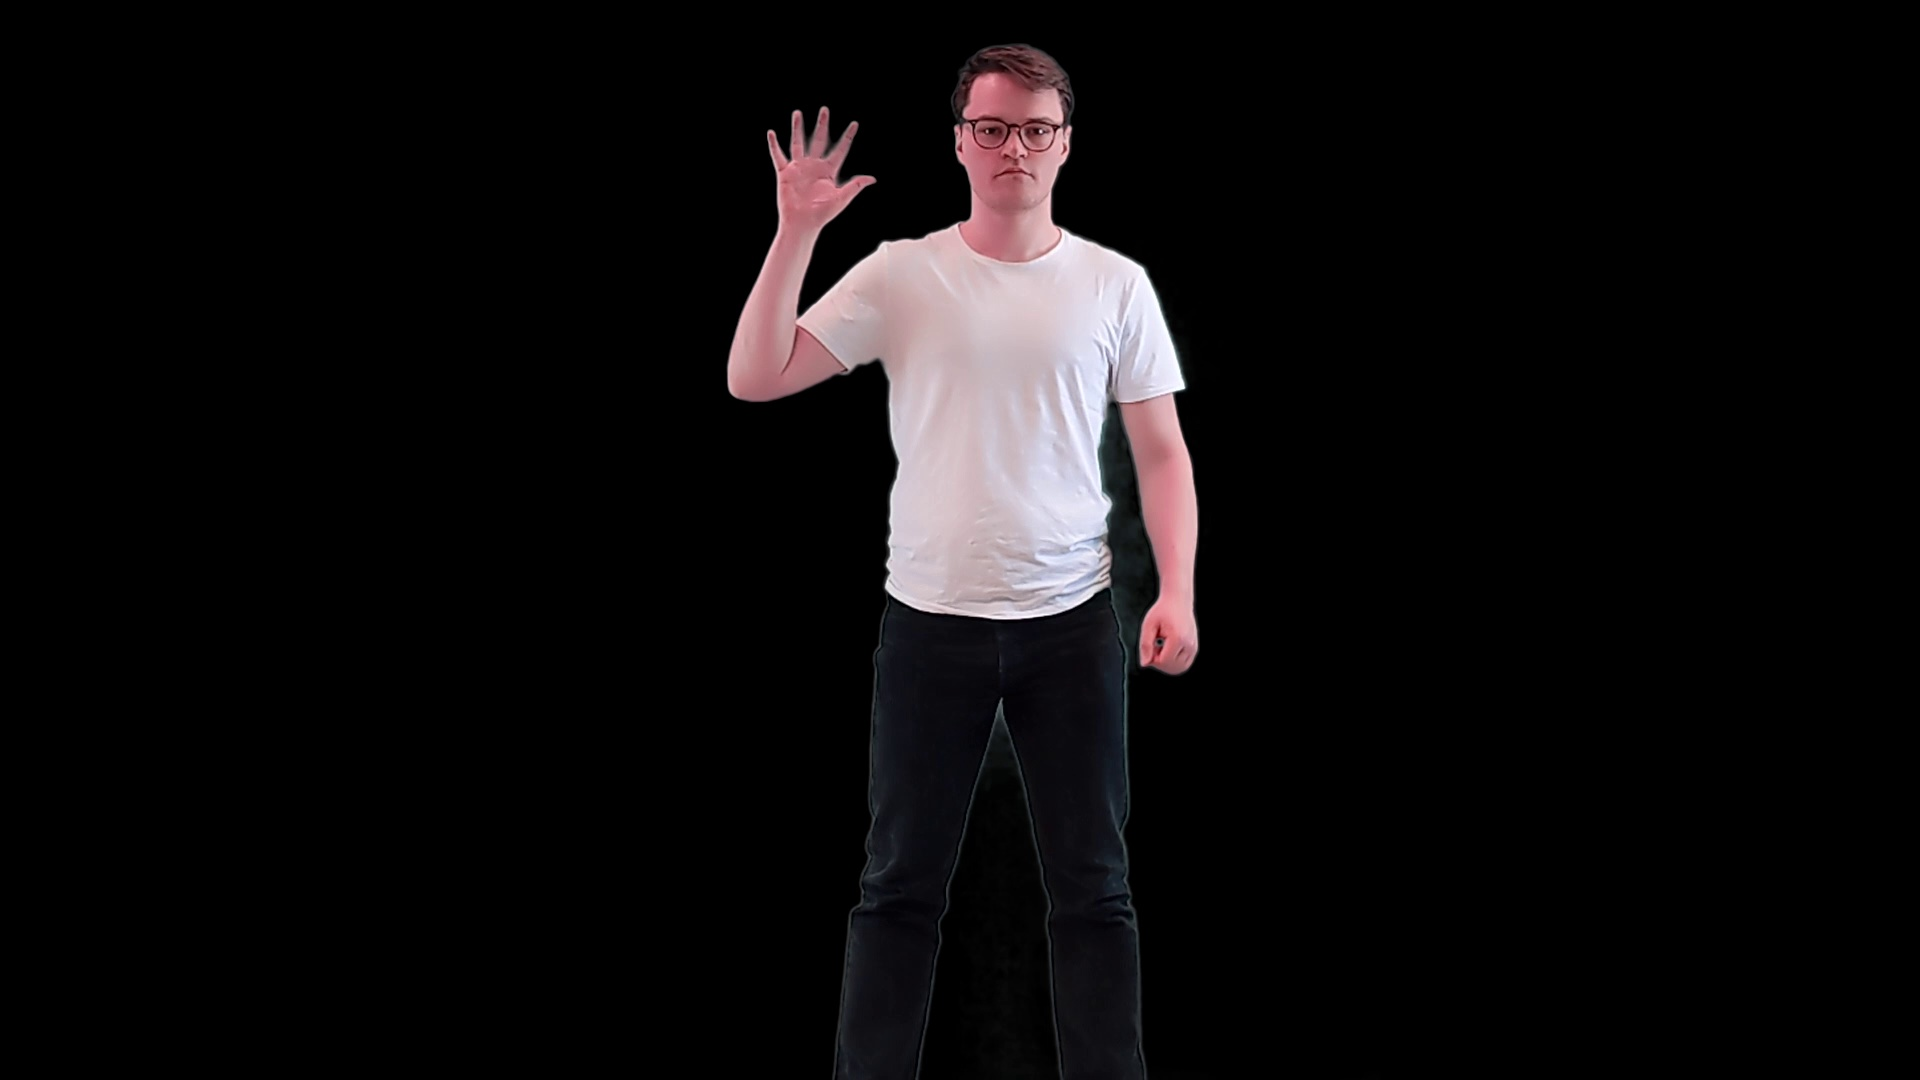
\includegraphics[width=0.6\textwidth]{img/video_frame_150/FG_Counting-Fingers_150.jpg}
    \caption{Frame 150 from the finger counting video}
    \label{fig:foreground_counting}
\end{figure}


\subsubsection{Person wearing a light clothing rocking back and forth}
See how well the algorithm performs on a person wearing light coloured clothing since some of the backgrounds will have lighter elements in them. How does this compare to the dark clothing?

\begin{figure}[H]
    \centering
    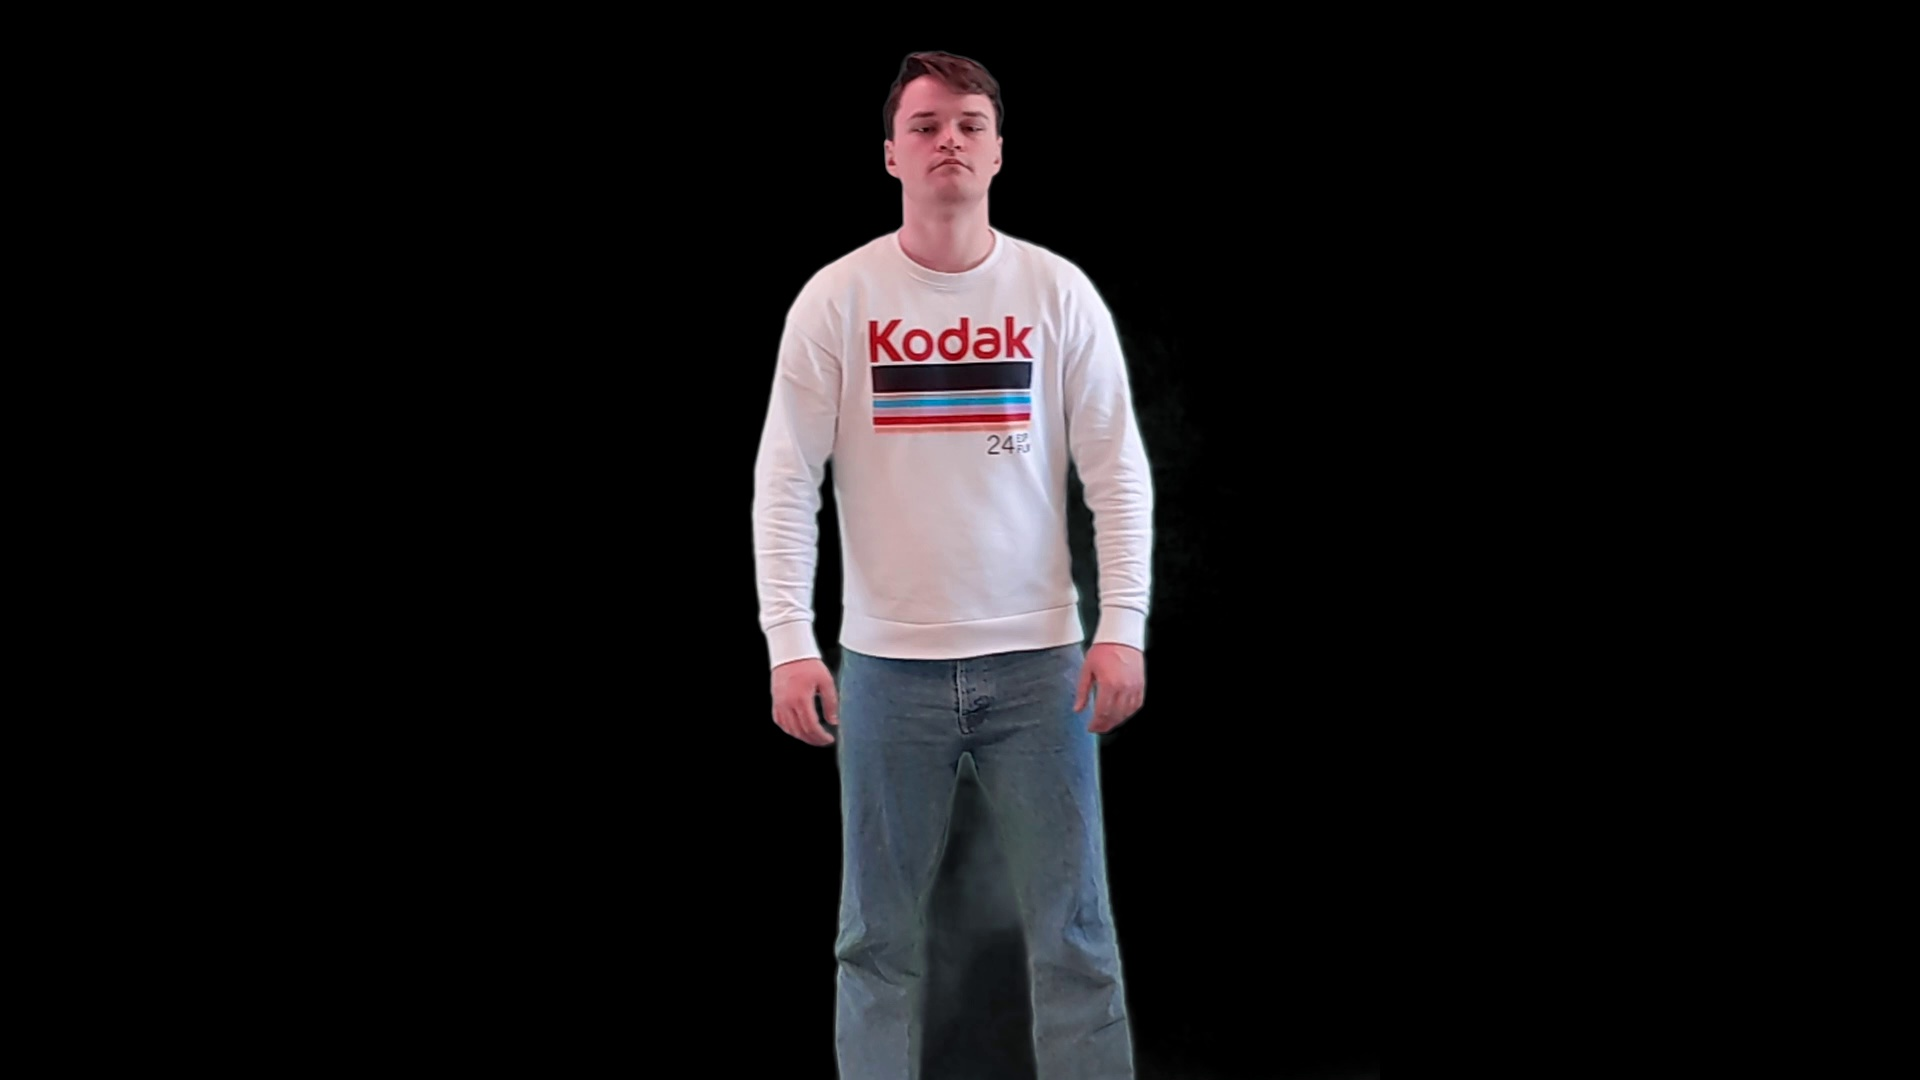
\includegraphics[width=0.6\textwidth]{img/video_frame_150/FG_Rocking-Light_150.jpg}
    \caption{Frame 150 from the light clothing video}
    \label{fig:foreground_light_clothing}
\end{figure}


\subsubsection{Person wearing a dark clothing rocking back and forth}
See how well the algorithm performs on a person wearing dark coloured clothing, since some of the backgrounds will have darker elements in them. How does this compare to the light clothing?

\begin{figure}[H]
    \centering
    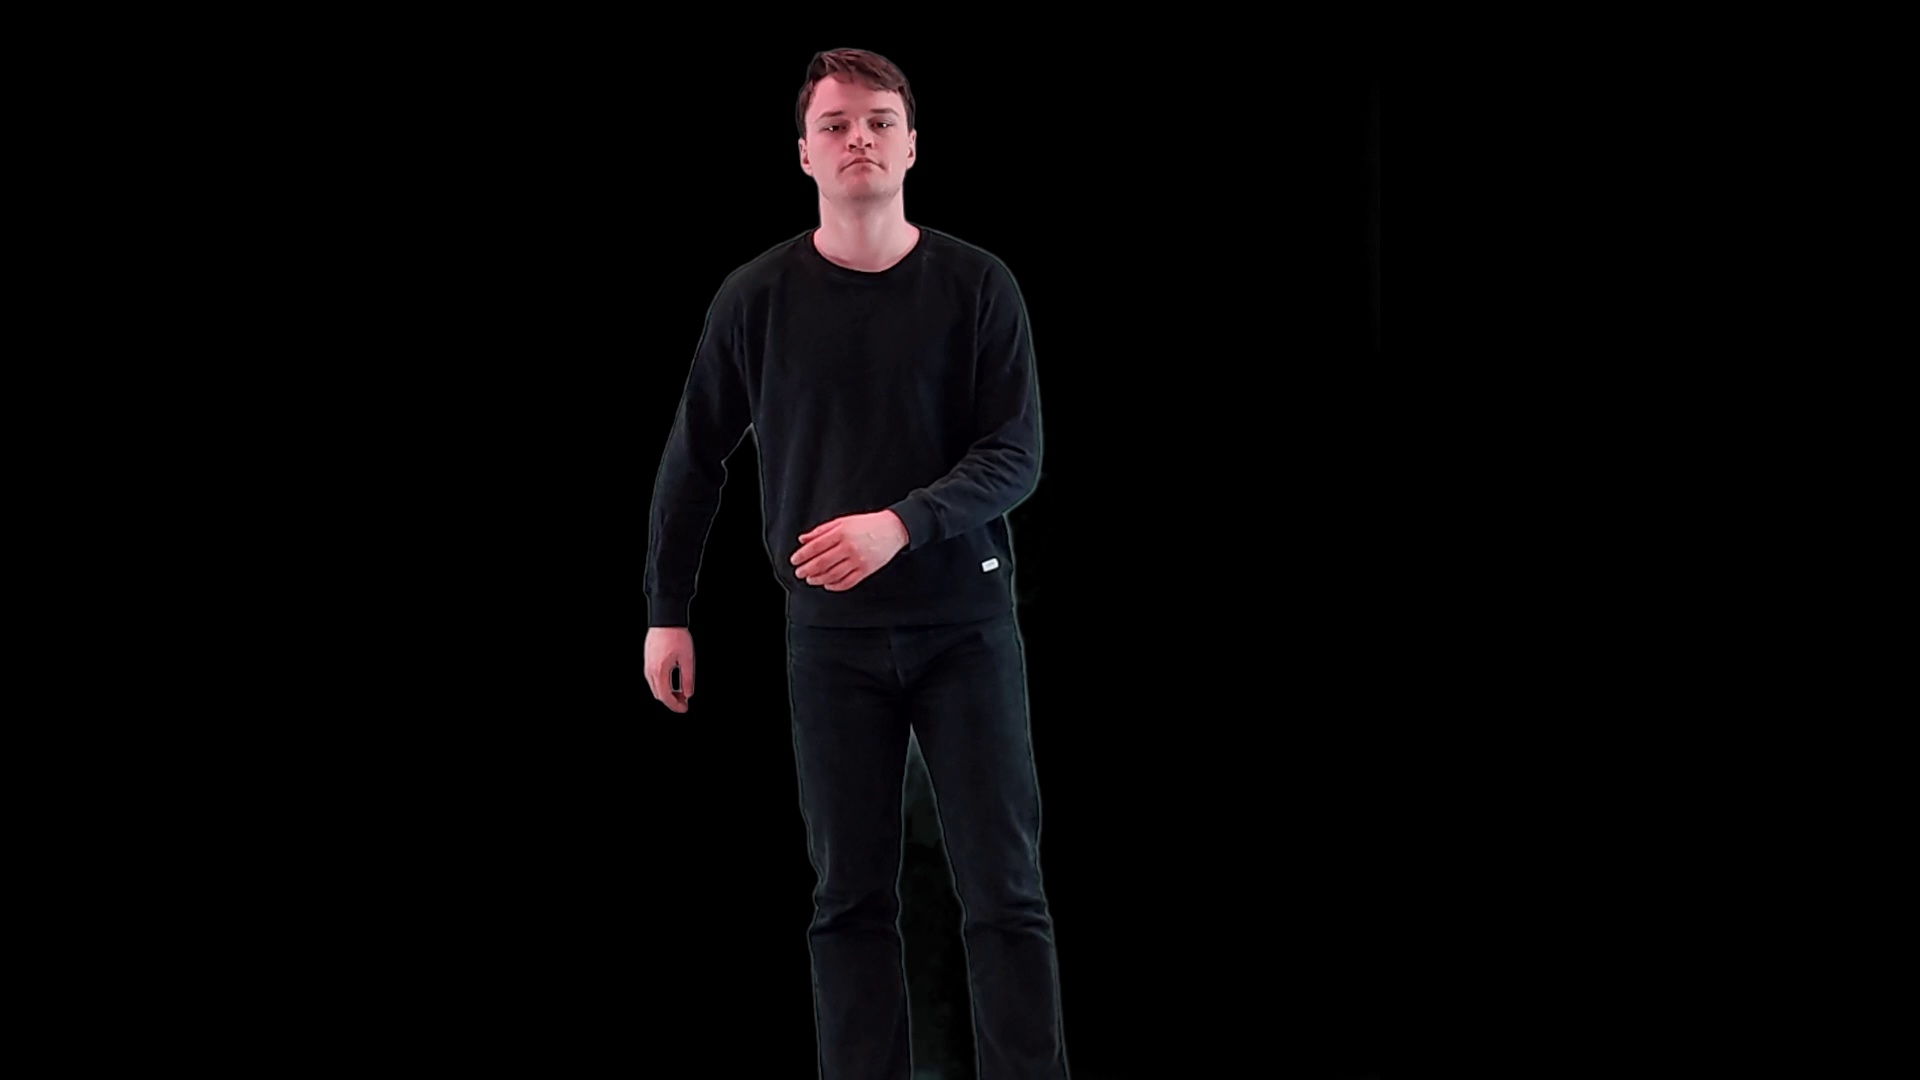
\includegraphics[width=0.6\textwidth]{img/video_frame_150/FG_Rocking-Dark_150.jpg}
    \caption{Frame 150 from the dark clothing video}
    \label{fig:foreground_dark_clothing}
\end{figure}


\subsubsection{Person displaying an object in their hands}
As we know from \autoref{sec:mlbfe}, the model is only trained on persons, but what happens if a person is holding an object, like a book? It is quite possible the \acrshort{mlbfe} is going to handle foreign objects in production. What will the \acrshort{mlbfe} do? Cut it out properly? Leave the object untouched?

\begin{figure}[H]
    \centering
    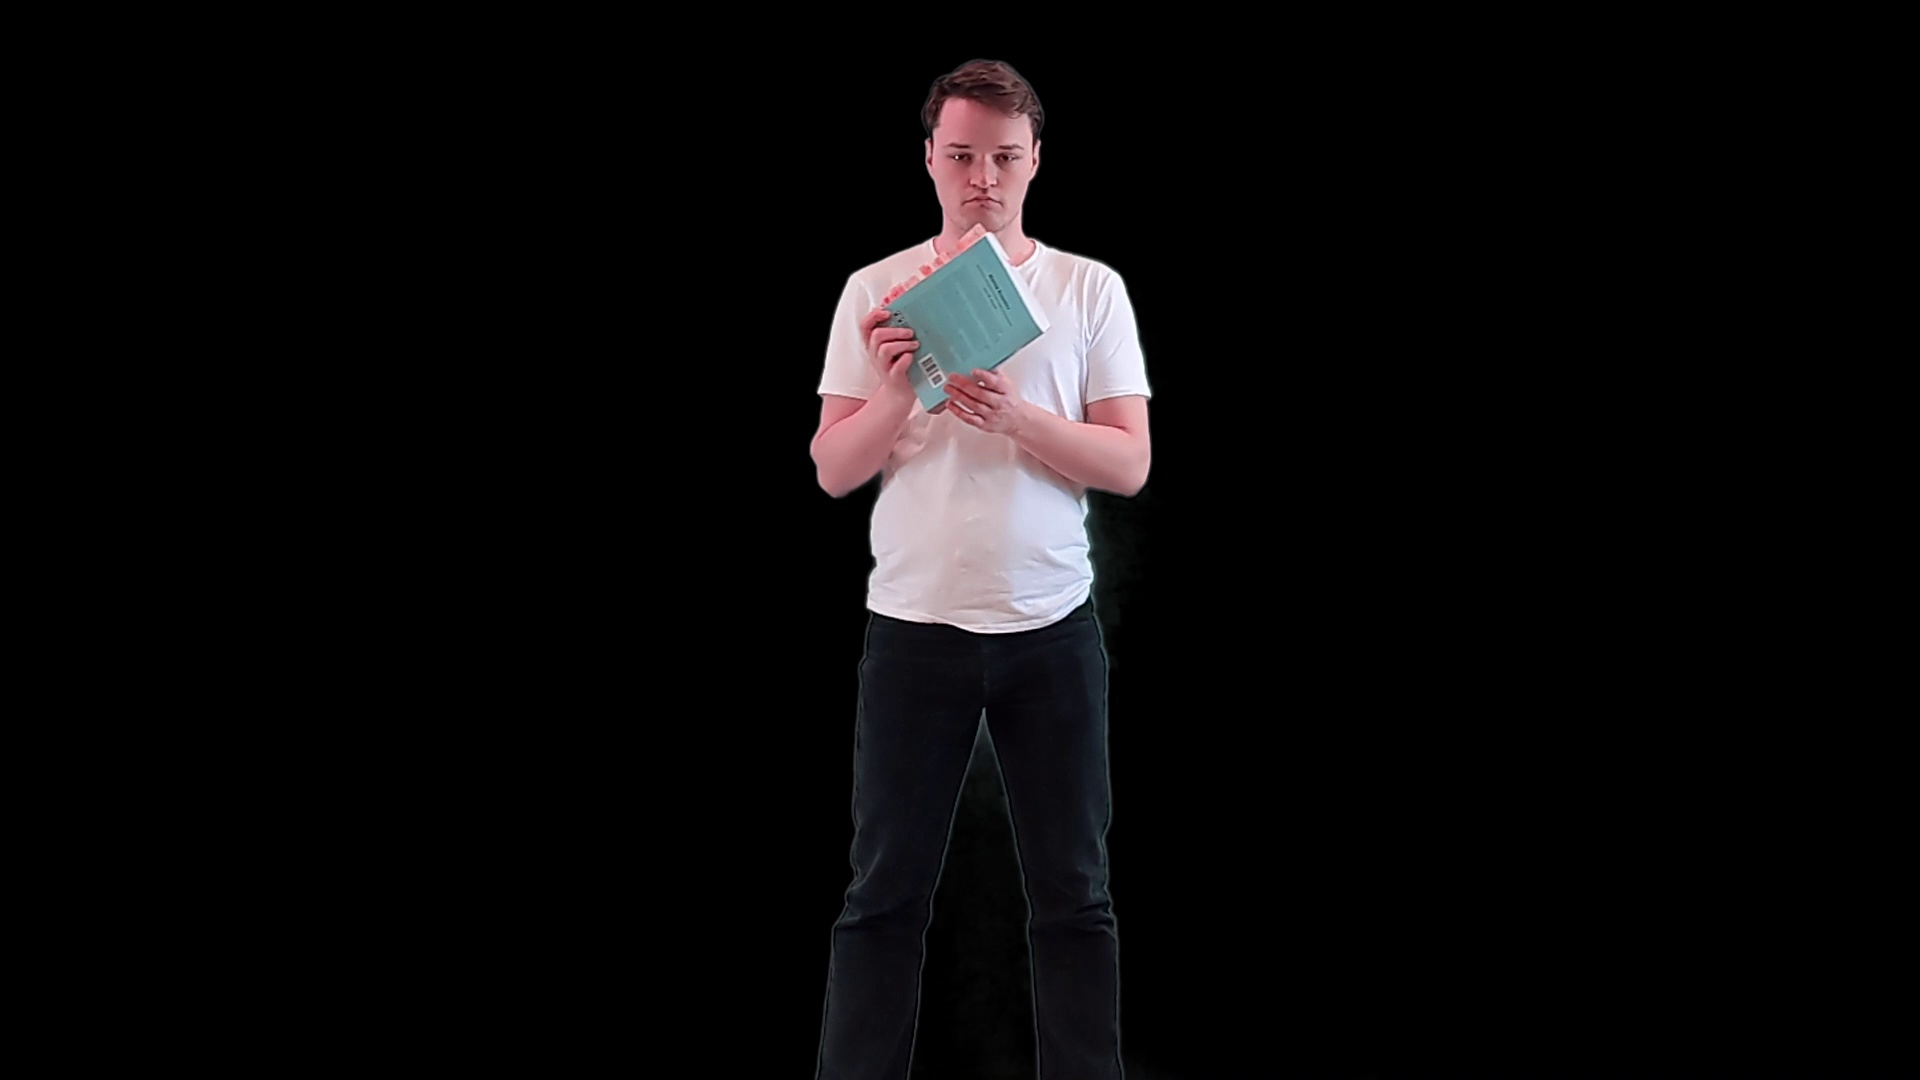
\includegraphics[width=0.6\textwidth]{img/video_frame_150/FG_Showing-Object_150.jpg}
    \caption{Frame 150 from the showing object video}
    \label{fig:foreground_showing_object}
\end{figure}

\subsection{Final Video List}
After the combinations of the different foregrounds and backgrounds, we get the final video list from \autoref{tab:video_list}.

\begin{table}[H]
    \centering
    \begin{tabular}{|c|p{4cm}|p{4cm}|} 
         \hline
         \textbf{Video} & \textbf{Foreground} & \textbf{Background} \\ [0.5ex] 
         \hline\hline
         1 & Showing Object & Complex \\
         \hline
         2 & Showing Object & Window \\
         \hline
         3 & Showing Object & White Wall \\
         \hline
         4 & Rocking Dark & Complex \\
         \hline
         5 & Rocking Dark & Window \\
         \hline
         6 & Rocking Dark & White Wall \\
         \hline
         7 & Rocking Light & Complex \\
         \hline
         8 & Rocking Light & Window \\
         \hline
         9 & Rocking Light & White Wall \\
         \hline
         10 & Counting Fingers & Complex \\
         \hline
         11 & Counting Fingers & Window \\
         \hline
         12 & Counting Fingers & White Wall \\
         \hline
    \end{tabular}
    \caption{}
    \label{tab:video_list}
\end{table}


\section{Measures}
\subsection{Objective measures}
The resulting videos from figure \ref{fig:videos}b (chroma key video) and \ref{fig:videos}d (machine learning video) will be statistically compared and reviewed head to head. The chroma key video will be our truth table, while the frame from the machine learning video will be our input. 

To make the computations easier, we will convert our frames to binary images in black and white, where the background is black and the silhouette extraction is white. We will be using Python to retrieve the objective measures discussed in \autoref{sec:objective_measurement} for each frame. Additionally, the mean of each objective measure will be calculated for each video for an general evaluation of the video in its entirety. The developed code can be found in \autoref{cha:appendix-github}.



\subsection{Subjective measures}\label{sec:system_subjective}
A group of participants will be given a questionnaire to collect the subjective measures of the quality of the resulting videos from the \acrshort{mlbfe} processed videos presented in \autoref{fig:videos}d. The questionnaire will map the demographic to map the age, gender, education and occupation, to see the coverage of low level human influencing factors and to see our representation of people. Afterwards, they will be asked some questions for each video. The questions, with answers, are listed in \autoref{tab:q1}, \autoref{tab:q2} and \autoref{tab:q1}.

\begin{table}[H]
    \centering
    \begin{tabular}{ |c|c| } 
         \hline
             \textbf{Question 1} & How satisfied are you with the quality of the silhouette extraction? \\
         \hline
             \textbf{Answer} & \begin{tabular}{c} Completely satisfied \\ Very satisfied \\ Moderately satisfied \\ Slightly satisfied \\ Not at all satisfied \end{tabular} \\
         \hline
    \end{tabular}
    \caption{Question and answers for question 1}
    \label{tab:q1}
\end{table}


\begin{table}[H]
    \centering
    \begin{tabular}{ |c|c| } 
         \hline
             \textbf{Question 2} & Did you notice any artefacts with the silhouette extraction? \\
         \hline
             \textbf{Answer} & \begin{tabular}{c} Extremely noticeable \\ Very noticeable \\ Moderately noticeable \\ Slightly noticeable \\ Not at all noticeable \end{tabular} \\
         \hline
    \end{tabular}
    \caption{Question and answers for question 2}
    \label{tab:q2}
\end{table}

\begin{table}[H]
    \centering
    \begin{tabular}{ |c|c| } 
         \hline
             \textbf{Question 3} & Do you think the artefacts were annoying? \\
         \hline
             \textbf{Answer} & \begin{tabular}{c} Extremely annoying \\ Very annoying \\ Moderately annoying \\ Slightly annoying \\ Not at all annoying \end{tabular} \\
         \hline
    \end{tabular}
    \caption{Question and answers for question 3}
    \label{tab:q3}
\end{table}


The participants will be able to answer the questions with a fitting five point Likert scale and also be able to add additional qualitative feedback in the end if wanted. 

The rating will be done using Google Forms. An export of the questionnaire is presented in \autoref{cha:appendix-questionnaire}. The videos have been implemented into the questionnaire as an unlisted YouTube video uploaded to a newly created account for the survey purpose. This has been done to prevent any targeted recommendations and other recommendations provided by the YouTube algorithms. 

The order of the videos presented in the questionnaire was decided by a shuffling the order of the videos through a randomising function, with the final order presented in \autoref{tab:order}. This was done to prevent the participants to see the same foreground videos after one another. Using this setup, we will be able to test on a lot of participants, which hopefully will yield a more fair and even result. 

\begin{table}[H]
    \centering
    \begin{tabular}{ |c|c|c|c|c|c|c|c|c|c|c|c|c| } 
         \hline
             \textbf{Video name number} & 1 & 2 & 3 & 4 & 5 & 6 & 7 & 8 & 9 & 10 & 11 & 12 \\
         \hline
             \textbf{Shuffled video order} & 10 & 9 & 3 & 7 & 6 & 2 & 1 & 12 & 8 & 4 & 11 & 5 \\
         \hline
    \end{tabular}
    \caption{Order of the videos in the questionnaire}
    \label{tab:order}
\end{table}

\section{Hardware}\label{sec:hardware}
\begin{table}[H]
    \centering
    \begin{tabular}{|p{2cm}|p{1.5cm}|p{3.5cm}|p{3cm}|} 
         \hline
         \textbf{What} & \textbf{Model} & \textbf{Specifications} & \textbf{Comment} \\ [0.5ex] 
         \hline\hline
         Video Camera Mobile Phone & Google Pixel 5 & Resolution: 1920x1080 \newline Codec: H.264, AAC, avc1 \newline Color Profile: (5-1-6) \newline Rec.601 (PAL) & Phone used to replicate the normal use case for the AdMiRe project \\
         \hline
         Editing machine & MacBook Air & 1.1GHz 4-core i5, 16GB RAM & Editing software: Final Cut Pro 10.6 \\
         \hline
         Machine learning machine & N.A. & 3.6GHz 8-core i7-7700, RTX A6000 & Running Ubuntu \\
         \hline
         Green Screen & Elgato & Extended: 148x180 cm & Feet get cut off \\
         \hline
         Ring Lights & Elgato & 2900-7000K, 2500 lm, 45W & One for left and right side. To remove shadows from green screen \\
         \hline
         Tripods & Any & N.A. & One for each ring light, and one for camera \\ [1ex] 
         \hline
    \end{tabular}
    \caption{Hardware specifications}
    \label{tab:harware}
\end{table}